%
%
%
%

\section{Method} \label{sec:method}
\begin{figure}
    \centering
    
\includegraphics[width=0.97\textwidth]{pipeline}
    \caption{Pipeline for applying zigzag persistence to temporal networks. Begin with an unweighted and undirected \textbf{temporal graph} where each edge is on at a point or interval of time. Create \textbf{graph snapshots} using a sliding window interval over the time domain. Create a sequence of \textbf{simplicial complexes} from the graphs and apply \textbf{zigzag persistence} to the union zigzag simplicial complexes.}
    \label{fig:pipeline}
\end{figure}

To apply zigzag persistence for studying temporal graphs, we use the pipeline shown in Fig.~\ref{fig:pipeline} which we describe more specifically here.
%
A temporal graph is a graph structure that incorporates time information on when edges and/or nodes are present in the graph. 
We will only be using the case of temporal information attributed to the edges in this work and assume nodes are included as part of an edge-induced subgraph.
Thus, our starting data is a graph $G = (V,E)$ where each edge $e$ has a collection of closed intervals $\mathcal{I}_e = \{I_{e,1}, \cdots, I_{e,k_e} \}$ associated to it for when that edge is active. 
Fitting with the previous section, we fix a collection of times $t_0\leq t_1 \leq \cdots \leq t_n$ and a choice of window size $w$.
Then $G_{i} = (V_i,E_i)$ is the graph induced by edges present within a window $[t_i-w/2,t_i+w/2]$. 
Please note that to ease notation, we are using subscripts $i$ for the graphs, but the graphs should be thought of as encoding information for the interval centered at $t_i$ and thus when computing persistence, the birth and death times are associated to the $t_i$'s rather than the $i$'s. 
Finally, we define $G_{i,i+1} = G_{i} \cup G_{{i+1}}$ to be the union of the two adjacent graphs.



While we can construct a zigzag filtration of graphs 
\begin{equation*}
G_{0} 
\hookrightarrow G_{0,1} 
\hookleftarrow G_{1} 
\hookrightarrow G_{1,2} 
\hookleftarrow G_{2} 
\hookrightarrow \ldots 
\hookleftarrow G_{{n-1}}  
\hookrightarrow G_{{n-1},{n}} 
\hookleftarrow G_{n}
%
\end{equation*}
this is not actually the zigzag we will be using since, as noted earlier, it is not flexible enough to find some of the loop structures needed in the later analysis. 
So, for any graph $G_i$ with vertex set $V_i \subseteq V$, we let $d_i$ be the shortest path distance on that graph. 
That is, $d_i:V_i \times V_i \to \R$ where $d_i(u,v)$ is the number of edges needed to get from vertex $u$ to vertex $v$. 
Fixing an $r\geq 0$, let $K_{i}^r:=R_r(V_i, d_i)$ be the Rips complex constructed from this distance information. 
First, we note that $K_i^0$ is the simplicial complex with only the vertex set $V_i$. 
When $r=1$, $K_i^1$ is the clique complex of the original graph $G_i$; where the 1-simplices are the same as that of the graph, but higher dimensional simplices are filled in when available. 
Then for higher $r$, we have more and more edges added to the original graph, so this construction is more complicated than simply treating the graph itself as a simplicial complex. 


Assuming we have similar notation for the union graph information ($d_{i,{i+1}}$, $K_{i,{i+1}}^r$, etc), we form a zigzag filtration by replacing $G_i$ with its Vietoris-Rips complex,
\begin{equation*}
 K_{0}^r %
\hookrightarrow K_{0,1}^r %
\hookleftarrow K_{1}^r %
\hookrightarrow K_{1,2}^r %
\hookleftarrow K_{2}^r %
\hookrightarrow \ldots 
\hookleftarrow K_{{n-1}}^r %
\hookrightarrow K_{{n-1},{n}}^r %
\hookleftarrow K_{n}^r. %
%
\end{equation*}
Finally, we compute the $p$-dimensional homology at each step and from there compute the zigzag persistence diagram. 
Our code uses the \texttt{Dionysus2} package \cite{Dionysus2} for this last step.
Again, be aware that the indices on the zigzag persistence points correspond to the $t_i$ value associated to the given complex.
%
%
%
%
%




%
%
%

%
%
%
%
%
%
%

%
%
%
%


%
%
%
%
%
%
%
%
%


\subsection{Example} 
\label{ssec:example}

\begin{figure}
     \centering
     %
     \begin{minipage}{0.64\textwidth}
         \centering
         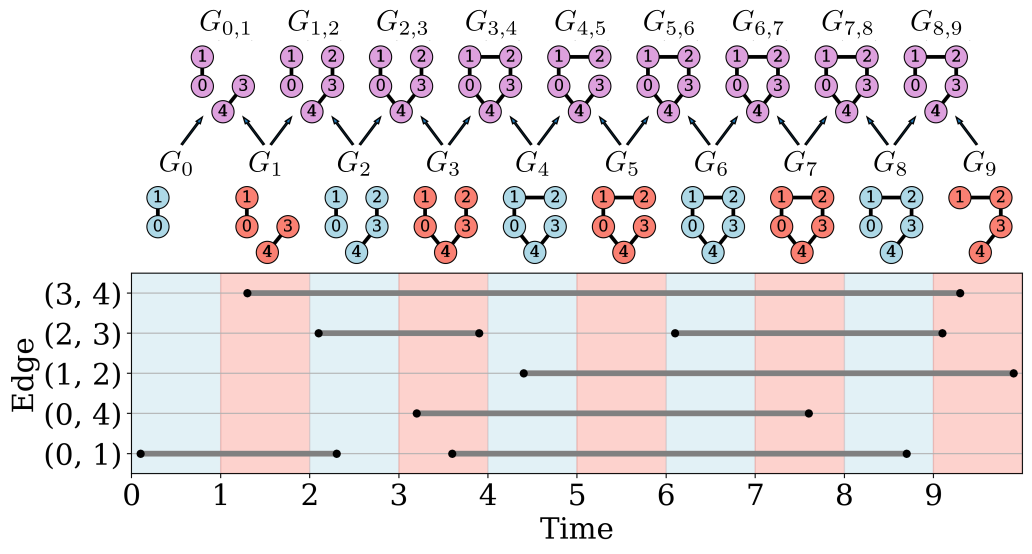
\includegraphics[width=\textwidth]{Figures/example_graph_sequence_and_intervals-ModifiedLabels}
     \end{minipage}
     \hfill
     \begin{minipage}{0.31\textwidth}
         \centering
         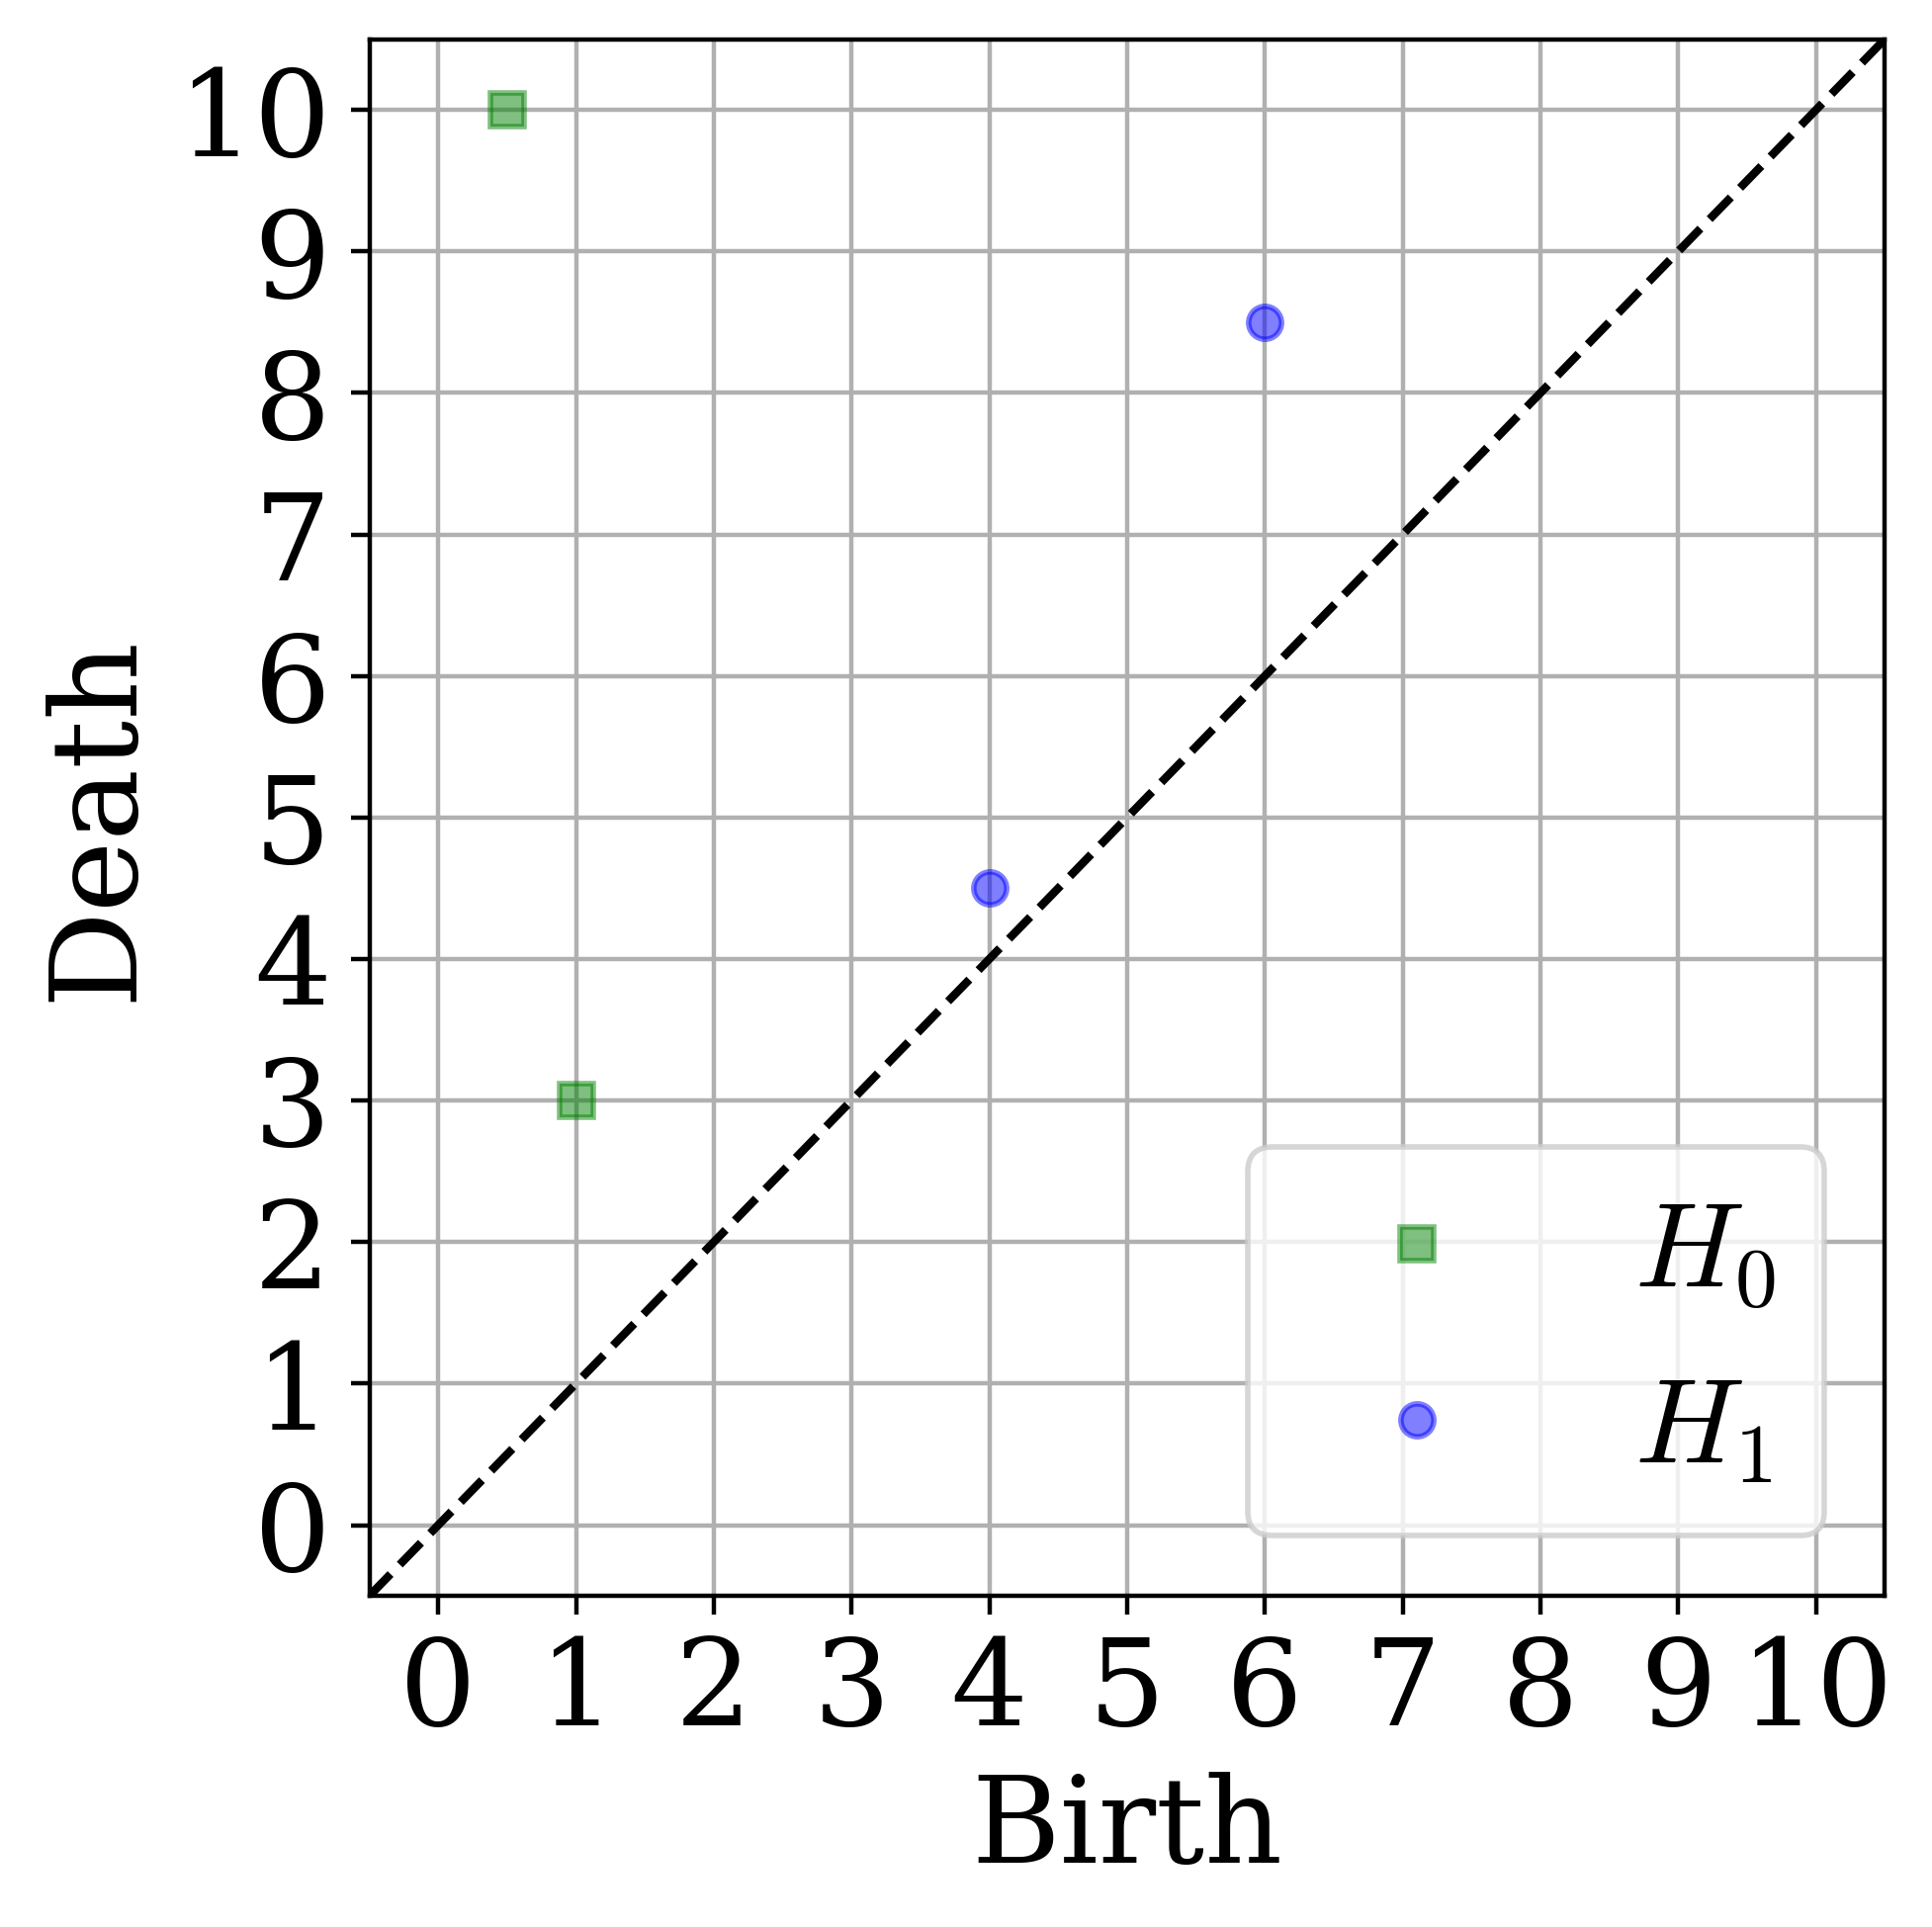
\includegraphics[width=\textwidth]{Figures/example_PD_dimension} 
     \end{minipage}


     %
     \caption{Example zigzag persistence applied to a simple temporal graph with temporal information stored for each edge as intervals. (Left) Edge intervals with sliding windows highlighted (alternating blue-red) with corresponding graphs and union graphs above. 
     (Right) Zigzag persistence diagram for both $H_0$ and $H_1$. The birth and death of a feature is encoded as the midpoint of the interval where the event happened. }
     \label{fig:example_zigzag_of_basic_temporal_graph}
\end{figure}

In the following simple example shown in Fig.~\ref{fig:example_zigzag_of_basic_temporal_graph}, we describe the method in more detail and show how to interpret the resulting zigzag persistence diagram.
In this example, we measure the changing structure of a simple 5-node cycle graph as edges are added and removed based on the temporal information. 
Fixing $r=1$, the simplicial complexes are exactly the same as the graphs $K_i = G_i$ as there are no cliques in this particular example.
The bottom left of Fig.~\ref{fig:example_zigzag_of_basic_temporal_graph}a shows the times associated to each edge, and the resulting graphs are shown above. 
In this notation, the subscripts correspond to the interval of time used to build the graphs. 
Then we have $w= 0.5$, and the centers of intervals are $t_0 = 0.5$, $t_1 = 1.5$, $\cdots$, $t_9 = 9.5$.
This results in intervals for graph $G_i$ of the form $(i,i+1)$ and intervals for the union graphs $G_{i,i+1}$ as $(i,i+2)$. 
At the end of the sliding windows, we consider the graph empty and set the death of any remaining homology features as the end time of the last window (i.e., $t=10$ for this example).

The resulting zigzag persistence diagram is shown in Fig.~\ref{fig:example_zigzag_of_basic_temporal_graph}b.
This persistence diagram shows the zero-dimensional and one-dimensional features as $H_0$ and $H_1$, respectively. There are two zero-dimensional features at persistence pairs $(1, 3)$ and $(0.5, 10)$. 
The later represents the connected component which appears at the first graph and lasts throughout the filtration. 
The other component is the piece consisting of vertices $3$ and $4$ which appears at union graph $G_{(0,2)}$, thus is associated to a birth at the midpoint of this interval occurring at 1. 


The one-dimensional feature (the cycle represented in $H_1$) is present twice in the persistence diagram. 
This is due to it first appearing in $G_{(3,5)}$ and then disappearing at $G_{(4,5)}$ with corresponding persistence pair $(4, 4.5)$. 
The cycle then reappears at $G_{(5,7)}$ and disappears at $G_{(8,9)}$ resulting in persistence pair at $(6,8.5)$. 

This example demonstrates how zigzag persistence captures the changing structure of temporal graphs at multiple dimensions. 
It is possible to also capture higher-dimensional structures using higher-dimensional homology, although we do not investigate this direction in this work.
In particular, it is not clear what higher dimensional homology would represent in the context of data coming from 1-dimensional graph structures.


